\subsubsection{Purpose}
The main user of the application who was correctly logged in the web application or the mobile one, can organize the appointments into his own calendar. The system provides the user the possibility to create, modify o delete any appointments that he has inserted.
In particular:
\begin{itemize}
	\item Create appointment: the user has to click on the specific date where he wants to add the new appointments, and inserted the information below:
	\begin{enumerate}
		\item Name of appointment;
		\item Start time;
		\item End time;
		\item Recurrence (optional);
		\item Means of transport.
	\end{enumerate}
	\item Modify appointment: the user simply click on the appointments that he has created so that he is able to update the information;
	\item Delete appointment: the user through the same gesture of "Modify appointment" can easly delete the appointment by clicking on the specific button.
\end{itemize}

\subsubsection{Scenario1}
Alice, a young business consultant, plans all her appointments through the Travlendar+ application. Every Wednesday, the company decides to organize a refresher course. For this reason, she needs to add this appointment to her calendar.
Alice through the calendar interface, click on the first day course and add the necessary information to create the appointment by using the form: event name, start time, end time, recurrence, means of transport. The system checks that the new appointment meets each requirement and asks Alice to confirm.
Once confirmed, the event is displayed in her list of appointments with the relevant means of transport to be used. Unfortunately, the company after a few days, deletes the refresher course, so Alice wants to delete the appointment from her calendar. Easily Alice accesses to the event and she modifies it. By clicking on the corresponding button, she deletes the event and all the saved recurrences. The system requires confirmation and so, the event is deleted from the calendar.

\subsubsection{Scenario2}
Bob, correctly signed up at Travlendar+, decides to check the appointments of the day through the calendar. While he’s scrolling through the appointment list, you notice that one of places of meetings was incorrectly entered. Easy, by clicking on the event, Bob is able to update the information. The system checks that the updated appointment meets each requirement. After calculating the time needed to reach the place of the appointment, the system creates a warning and it warns Bob that the travel time between the previous and the updated event is not enough to reach the place of the appointment. However, the system asks Bob if he wants to confirm or update the event.
He doesn’t choose to update the event, so changes are not made.
Bob accesses to the event and he modifies it again, but in this case, he deletes the event by clicking on the specific button. The system requires confirmation and the event is deleted form the calendar.

\begin{table}
\centering
	\begin{tabular}{|c||p{0.6\textwidth}|}
		\hline
		Name & Create appointment \\ \hline
		Actors & User \\ \hline
		Assumption & The user need to insert a new appointment in his personal calendar \\ \hline
		Pre-Conditions & \begin{itemize}
			\item The user has successfully signed to the system
			\item The user has already opened the window with the insertion form.
		\end{itemize} \\ \hline
		Flow of events & \begin{enumerate}
			\item The user creates a new appointment by inserting all the information needed in order to adding a new event correctly in his own calendar.
			\item The system check into the calendar if the location of the appointment is reachable in the allotted time or if the event is overlapping with other appointment.
			\item The user is informed by a warning message about the actual validation of the appointment.
			\item The user have to confirm o reject the insertion of the appointment
		\end{enumerate} \\ \hline
		Post-Conditions & The appointment of the user has been stored to the system in the event that he has confirmed the inclusion. \\ \hline
		Exception & An internal system error makes impossible to store the reservation data. The user is notified of the error \\ \hline		
	\end{tabular}
\caption{Use case for appointments handling}
\label{usecase_app}
\end{table}

\begin{figure}[H]
	\centering
	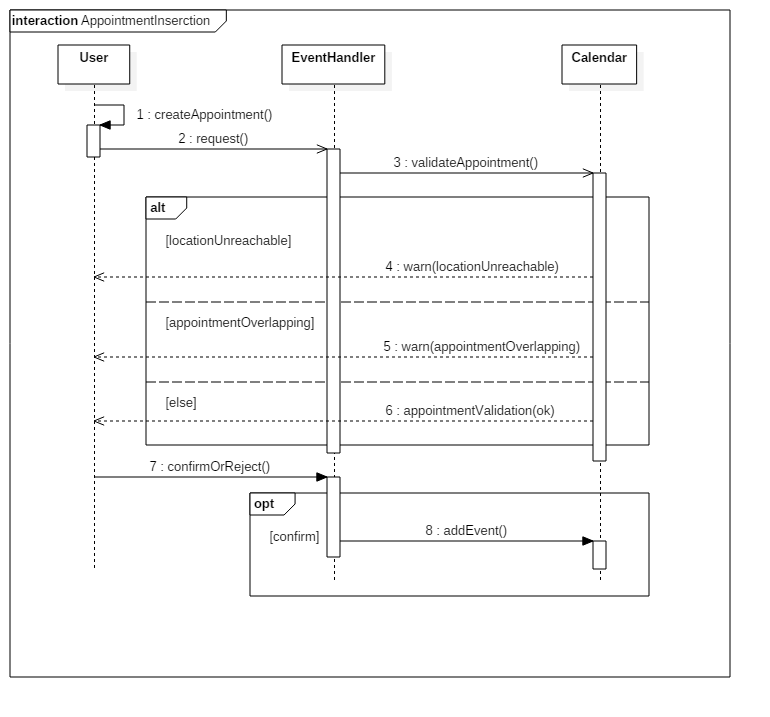
\includegraphics[width=6in]{./diagrams/AppointmentInserction.png}
	\caption{Sequence Diagram: Create Appointment}
	\label{fig:SequenceAddApp}
\end{figure}